\chapter{Results}\label{Sec:Results}

In this chapter, we discuss the results and discussion phase. It explains the results of all the 192 experiments on our dataset. Also, How we assess our model design. We discuss some aspect related to our results.

In this section we explain the results of all the 192 experiments in our dataset. We measure the results using the overall accuracy, then measure the performance accuracy of the model per class (meter). We start by presenting the results for every combination, and then discuss our findings relating to the topic.

As explained in Section~\nameref{Ch:Model_Training} we have a set of combinations requiring exploration. Most of our results therefore involve a combination. These are explored below:

\begin{enumerate}

 \item Three data representations, \textit{binary}, \textit{one-hot}, and \textit{two-hot}, are represented as \textbf{\textit{BinE, OneE, TwoE}} respectively.
 \item Two types of model loss functions, \textbf{\textit{Weighting loss and no Weighting loss}}, are represented as \textbf{\textit{(1 and 0)}} respectively.
 \item The Number of layers is represented as \textbf{\textit{nL}}; for example, 7 layers are 7L.
 \item The Number of cell units is represented as \textbf{\textit{nU}}; for example, 82 units is 82U.

\end{enumerate}

Therefore, if we need to explain a set of combinations, we write (4L, 82U, 0), which means 4 layers, 82 units, and no weighted loss function. Many figures are provided, all of which explain specific perspectives on the results .

\section{Overall Accuracy}

We present the overall accuracy score of the 16 neural networks configurations and at each of the 12 data representations (y- and x-axis respectively) in Figure~\ref{Fig:ArabicModelsResults}. The x-axis is divided into 4 strips corresponding to the 4 combinations of trimming and diacritical parameters. Each strip includes the 3 different encoding values. Each point on the figure represents the overall accuracy score of one of the 192 experiments (some values are too small, and hence omitted from the figure). To explain the figure, we take as an example the most-left vertical list of points that represent the 16 experiments of the full (no trimming), diacritics, and \textit{binary} encoding dataset representation. For each rug plot, the highest (Bi)LSTM accuracies are labeled differently, as circle and square respectively; and the network configuration of both is listed at the top of the rug plot.

To explain the figure, we take as an example the most-left vertical rug plot, which corresponds to (0T, 1D, BinE) data representation. The accuracies of the best (Bi)LSTM are 0.9025 and 0.7978 respectively. The configuration of the former is (7L, 82U, 0W). Among all the 192 experiments, the highest accuracy is 0.9638 and is possessed by (4L, 82U, 0W) network configuration on (1T, 0D, BinE) data representation.



\begin{figure}[!t]

	\input{./Figures/Ch_7_Results/Fig_Overall_Score.tex}
	\caption{Overall accuracy of the 192 experiments plotted as 2 vertical rug plots (for the 12 different data representations: $\left\{\mathit{Trimming},\ \mathit{No Trimming} \right\} \times \left\{\mathit{Diacritics},\ \mathit{No Diacritics} \right\} \times \left\{\mathit{OneE},\ \mathit{BinE},\ \mathit{TwoE}\right\}$), each represents 16 exp. (for the 16 different network configurations: $\left\{7L,\ 4L\right\} \times \left\{82U,\ 50U\right\} \times \left\{0W, 1W\right\} \times \left\{LSTM,\ BiLSTM\right\}$). For each rug plot the best model of each of the four cell types ---(Bi)LSTM labeled differently. Consistently, BiLSTM was the winner, and its network configuration parameters are listed at the top of each rug plot.}~\label{Fig:ArabicModelsResults}
\end{figure}


%%%%%%%%%%%%%%%%%%%table of results here


\begin{table}[!h]
	\centering
	\begin{tabular}{c c c c c c c c c}
		\hline
		\textbf{Experiment Id} & \textbf{Accuracy}  &  \textbf{Encoding Types} & \textbf{Diacritic} &\textbf{Trimming}& \textbf{Cell Type} & \textbf{Layers} & \textbf{Units} & \textbf{Weighted Loss}\\
		
		\hline
1 & 0.963847 & \textit{Binary} & D0 & T0 & BI-LSTM & \textit{3} &  \textit{82} & \textit{W0} \\
2 & 0.962883 & \textit{Two-Hot} & D0 & T0 & BI-LSTM & \textit{3} &  \textit{50} & \textit{W1}\\
3 & 0.962721 & \textit{Two-Hot} & D0 & T0 & BI-LSTM & \textit{3} &  \textit{82} & \textit{W0} \\
4 & 0.962105 & \textit{Binary} & D0 & T0 & BI-LSTM & \textit{6} &  \textit{50} & \textit{W1} \\
5 & 0.961955 & \textit{Binary} & D0 & T0 & BI-LSTM & \textit{6} &  \textit{82} & \textit{W0} \\
6 & 0.961189 & \textit{Binary} & D0& T0 & BI-LSTM & \textit{3}  &  \textit{82}& \textit{W1} \\
7 & 0.960404 & \textit{Binary} & D0 & T0 & BI-LSTM & \textit{3} &  \textit{50} & \textit{W0} \\
8 & 0.959949 & \textit{Two-Hot} & D0 & T0 & BI-LSTM & \textit{3} &  \textit{50} & \textit{W0} \\
9 & 0.957686 & \textit{Binary} & D0 & T0 & BI-LSTM & \textit{3} &  \textit{50} & \textit{W1} \\
10 & 0.955668 & \textit{Binary} & D0 & T0 & BI-LSTM & \textit{6} &  \textit{50} & \textit{W0} \\
\hline
	\end{tabular}
	\caption{Top ten experiments results}\label{Tab:Exp_Results}
\end{table}


\section{Data Representation Effects}

In this section we will explain the effect of the 12 data representation techniques explained previously.

\begin{enumerate}
 \item \textbf{Trimming Effect:} The effect of trimming (removing the small classes from the training cycle) can be observed if we fix the other two parameters, diacritic and encoding. The score with trimming is consistently higher than that with no trimming, e.g. by looking at the two unshaded strips, the score at (1T, 0D, TwoE) is 0.9629, while that at (0T, 0D, TwoE) is 0.9411. The only exception, with very little difference, is (1T, 1D, BinE) vs. (0T, 1D, BinE). We need to highlight that this effect is logical, as the training will have fewer classes with a huge amount of data for these classes.
 \item \textbf{Diacritics Effect}
 \begin{itemize}
 \item \textit{Without Trimming:} The effect of diacritics is obvious only with no trimming (the two left strips of the figure) where, for each encoding, the accuracy score is higher for diacritics than no diacritics.
 \item \textit{With Trimming:} The diacritics have no effect other than in the \textit{one-hot} encoding, while other encoding has no effect on the model performance. This result is inconsistent with that anticipated, from the effect of diacritics. It is believed that this result is an artifact due to the small number of network configurations.

 \end{itemize} 
 \item \textbf{Encoding Effect:} The effect of encoding is clear; by looking at each individual strip, \textit{overall accuracy score is consistently highest for \textit{two-hot} then \textit{one-hot} then \textit{binary}} the only exception is (1T, 0D, BinE) which performs better than the other two encodings. It seems that \textit{two-hot} encoding makes it easier for networks to capture the patterns in data. However, we anticipate that there is a particular network architecture for each encoding that can capture the same pattern while yielding the same score.
\end{enumerate}




\section{Network Configurations Effects}

This section is to comment on the effect of the network configurations parameters.
\begin{itemize}

\item \textbf{Cell Type}: It is clear that BI-LSTM (large circle) has the highest accuracy score for each data representation. It is always higher than the highest score of the LSTM model (large square). This is what we expected; the more complex architecture, the more results we can achieve. However, we need to mention that the BI-LSTM is slower than LSTM in overall running time for all experiments, and also consumes much more resources than LSTM cell.
\item \textbf{Layers Number}: Layers Number: As explained in Section~\nameref{Sec:Deep_Learning_Background}, the idea behind the deep neural network comes from the multi-layers which make the network learn more details. Hence, the more complex the network (more layers), the more results we can achieve. In our experiments,therefore, we can show that 7 layers achieved higher scores than 4 layers. There is an exception for the trimming data without diacritics in (1T, 0D, BinE) and (1T, 0D, TwoE). The straightforward interpretation for this is that the reduction in dataset size occurred by trimming and no diacritics, which required a less complex network. Hence, reducing the complexity of our problem (the number of layers will not be effective).
\item \textbf{Cell Units and Weighting Loss}: We cannot ascertain a consistent effect based on the number of cell units or the weighting loss, but we must mention that the highest results were achieved using both the highest cell units (82) and the weighted loss.

\end{itemize}



\section{Per-Class (Meter) Accuracy}

In this section, we explore the accuracy of each class. This addresses how our model can detect every class separately. It is similar to accuracy (see above) but involves per-class calculation. It is useful to check, as it will show how the model may understand each class, and which classes our model was unable to classify. 

Similar to the previous section, we employ four combinations of \textit{trimming and diacritic}: we investigate which models achieved the best results. We take the best four models (the first involve \textit{two-hot} encoding, and the fourth \textit{binary} encoding) from Figure~\ref{Fig:ArabicModelsResults}, which represents the overall accuracy and shows the results of the per-class accuracy for each one.

In Figure~\ref{Fig:Results_Per_Class} we have the previous four models display the per-class accuracy. We ordered The class names based on their data size per class. It explained previously in Figure~\ref{Fig:Data_Size_Distribution} with the same order. If we compare the results for the four models accuracy scores were around 95\% in Figure~\ref{Fig:ArabicModelsResults} and the per-class accuracy, we will find only 6 classes (which have around 80\% of the total datasets) are around this value. But there are significant drops for some classes which make the figures line has dropped in the results.


Figure~\ref{Fig:Results_Per_Class} shows the relation between the model accuracy results per-class and the dataset size per class; however, this trend was expected to be fixed from the weighted loss which has an inconsistent effect on the weighting loss for all the models. This inconsistent effect shows we need a new design which has an function which can solve this trending issue. The overall accuracy can be increased after trimming but there will be a gap between the accuracy per class the size of the data per class as the dataset is not balanced. Moreover, we can repeat this experiment, ensuring all classes have an equal size; we can therefore show the accuracy without the issue of data unbalance.This is developed in Section~\nameref{Sec:Discussion}.


\begin{figure}[!t]
 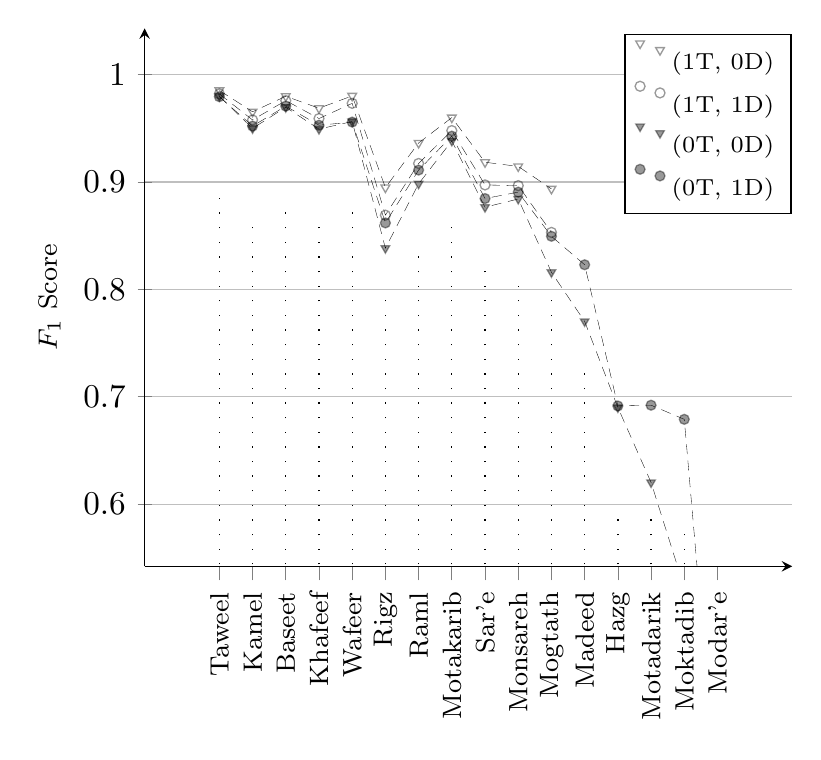
\begin{tikzpicture}[scale=1.2]
  \begin{axis}[
    axis x line = bottom,
    axis y line = left,
    ymajorgrids = true,
    ybar,
    enlargelimits=0.15,
    legend style={at={(0.87,0.99)},
      anchor=north,legend columns=1},
    ylabel={$F_{1}$ Score},
    ylabel style = {font=\footnotesize},
    symbolic x coords={Taweel, Kamel, Baseet, Khafeef, Wafeer, Rigz, Raml, Motakarib, Sar'e, Monsareh, Mogtath, Madeed, Hazg, Motadarik, Moktadib, Modar'e},
    xtick=data,
    xticklabel style = {font=\footnotesize},
    nodes near coords align={vertical},
    x tick label style={rotate=90, anchor=east},
    bar width=2pt,
    ymin=0.6,
    ]

    % trimmed no-diacritic (Empty Triangle)
    \addplot[mark=triangle, every mark/.append style={rotate=180},
    thin, only marks, mark size=1.5pt, point meta=explicit symbolic, opacity=0.4]
    coordinates {
      (Taweel,     0.9851172524158307)       
      (Kamel,      0.9652475629233903)       
      (Baseet,     0.9796481833964317) 
      (Khafeef,    0.9685310147936672)       
      (Wafeer,     0.9800042695509855)       
      (Rigz,       0.8946829393189383)       
      (Raml,       0.9361911800936191)       
      (Motakarib,  0.959795491517546 )       
      (Sar'e,      0.9182454343744668)       
      (Monsareh,   0.914378612716763 )       
      (Mogtath,    0.8934631432545201)       
      % Damn Trick; the first \addplot must have all the x ticks; otherwise
      % the following 4 ticks will not appear on the x-axis.
      (Madeed,     0)  
      (Hazg,       0)
      (Motadarik,  0) 
      (Moktadib,   0) 
      (Modar'e,    0)
    };

    % trimmed diacritic (Empty Circle)
    \addplot[mark=o, thin, only marks, mark size=1.5pt, point
    meta=explicit symbolic, opacity=0.4]
    coordinates{
      (Taweel,    0.9818557817770008)       
      (Kamel,     0.9576166230906838)       
      (Baseet,    0.9756393621028839) 
      (Khafeef,   0.9589173825980233)       
      (Wafeer,    0.97306361268686  )       
      (Rigz,      0.8690169840452907)       
      (Raml,      0.9171277587814735)       
      (Motakarib, 0.9476956555529649)       
      (Sar'e,     0.8971480834788392)       
      (Monsareh,  0.8964889939967255)       
      (Mogtath,   0.852965982569581 )       
    };



    % full no-diacritic (Full Triangle)
    \addplot[mark=triangle*, every mark/.append style={rotate=180},
    thin, only marks, mark size=1.5pt, point meta=explicit symbolic, opacity=0.4]
    coordinates {
      (Taweel,     0.9797117984076986)       
      (Kamel,      0.9497651482802794)       
      (Baseet,     0.9694416914436736) 
      (Khafeef,    0.9490905591377153)       
      (Wafeer,     0.9561501167175435)       
      (Rigz,       0.8382501685772085)       
      (Raml,       0.8982087708462013)       
      (Motakarib,  0.9381081512202903)       
      (Sar'e,      0.8764296156161321)       
      (Monsareh,   0.884060552092609 )       
      (Mogtath,    0.8158338012352612)       
      (Madeed,     0.7701375245579568 )  
      (Hazg,       0.690017513134851  )
      (Motadarik,  0.6202661207778916 ) 
      (Moktadib,   0.5223880597014925 ) 
      (Modar'e,    0.21428571428571427)
    };

    % full diacritic (Full Circle)
    \addplot[mark=*, thin, only marks, mark size=1.5pt, point
    meta=explicit symbolic, opacity=0.4]
    coordinates {
      (Taweel,    0.9792390538251331)       
      (Kamel,     0.951906768069158 )       
      (Baseet,    0.9704723593082569) 
      (Khafeef,   0.9527113852480082)       
      (Wafeer,    0.9556124626547161)       
      (Rigz,      0.8617761929020207)       
      (Raml,      0.9109545163356824)       
      (Motakarib, 0.9425525143220879)       
      (Sar'e,     0.884472886493769 )       
      (Monsareh,  0.8904428904428904)       
      (Mogtath,   0.8493552168815944)       
      (Madeed,    0.8228498074454429)  
      (Hazg,      0.6914546640574037)
      (Motadarik, 0.6921529175050303) 
      (Moktadib,  0.6790123456790124) 
      (Modar'e,   0.3225806451612903)
    };

    \legend{
      {\scriptsize (1T, 0D)},
      {\scriptsize (1T, 1D)},
      {\scriptsize (0T, 0D)},
      {\scriptsize (0T, 1D)},
    }

    % Dotted line
    \draw[loosely dotted] (axis cs:Wafeer,    0) -- (axis cs:Wafeer,     0.8800042695509855);
    \draw[loosely dotted] (axis cs:Monsareh,  0) -- (axis cs:Monsareh,   0.814378612716763 );
    \draw[loosely dotted] (axis cs:Mogtath,   0) -- (axis cs:Mogtath,    0.7934631432545201);
    \draw[loosely dotted] (axis cs:Motakarib, 0) -- (axis cs:Motakarib,  0.859795491517546 );
    \draw[loosely dotted] (axis cs:Kamel,     0) -- (axis cs:Kamel,      0.8652475629233903);
    \draw[loosely dotted] (axis cs:Taweel,    0) -- (axis cs:Taweel,     0.8851172524158307);
    \draw[loosely dotted] (axis cs:Sar'e,     0) -- (axis cs:Sar'e,      0.8182454343744668);
    \draw[loosely dotted] (axis cs:Raml,      0) -- (axis cs:Raml,       0.8361911800936191);
    \draw[loosely dotted] (axis cs:Rigz,      0) -- (axis cs:Rigz,       0.7946829393189383);
    \draw[loosely dotted] (axis cs:Khafeef,   0) -- (axis cs:Khafeef,    0.8685310147936672);
    \draw[loosely dotted] (axis cs:Baseet,    0) -- (axis cs:Baseet,     0.8796481833964317);
    \draw[loosely dotted] (axis cs:Moktadib,  0) -- (axis cs:Moktadib,   0.5790123456790124);
    \draw[loosely dotted] (axis cs:Madeed,    0) -- (axis cs:Madeed,     0.7228498074454429);
    \draw[loosely dotted] (axis cs:Hazg,      0) -- (axis cs:Hazg,       0.5914546640574037);
    \draw[loosely dotted] (axis cs:Modar'e,   0) -- (axis cs:Modar'e,    0.2225806451612903);
    \draw[loosely dotted] (axis cs:Motadarik, 0) -- (axis cs:Motadarik,  0.5921529175050303);



    % connecting a models F_1s
    % Full Triangle
    \draw[line width=0.1pt, densely dashed]
    (axis cs:Taweel,     0.9797117984076986)
    -- (axis cs:Kamel,      0.9497651482802794)
    -- (axis cs:Baseet,     0.9694416914436736)
    -- (axis cs:Khafeef,    0.9490905591377153)
    -- (axis cs:Wafeer,     0.9561501167175435)
    -- (axis cs:Rigz,       0.8382501685772085)
    -- (axis cs:Raml,       0.8982087708462013)
    -- (axis cs:Motakarib,  0.9381081512202903)
    -- (axis cs:Sar'e,      0.8764296156161321)
    -- (axis cs:Monsareh,   0.884060552092609 )
    -- (axis cs:Mogtath,    0.8158338012352612)
    -- (axis cs:Madeed,     0.7701375245579568)
    -- (axis cs:Hazg,       0.690017513134851 )
    -- (axis cs:Motadarik,  0.6202661207778916)
    -- (axis cs:Moktadib,   0.5223880597014925)
    -- (axis cs:Modar'e,    0.2142857142857142);

    % Full Circle
    \draw[line width=0.1pt, densely dashed]
    (axis cs:Taweel,     0.9792390538251331)
    -- (axis cs:Kamel,      0.951906768069158 )
    -- (axis cs:Baseet,     0.9704723593082569)
    -- (axis cs:Khafeef,    0.9527113852480082)
    -- (axis cs:Wafeer,     0.9556124626547161)
    -- (axis cs:Rigz,       0.8617761929020207)
    -- (axis cs:Raml,       0.9109545163356824)
    -- (axis cs:Motakarib,  0.9425525143220879)
    -- (axis cs:Sar'e,      0.884472886493769 )
    -- (axis cs:Monsareh,   0.8904428904428904)
    -- (axis cs:Mogtath,    0.8493552168815944)
    -- (axis cs:Madeed,     0.8228498074454429)
    -- (axis cs:Hazg,       0.6914546640574037)
    -- (axis cs:Motadarik,  0.6921529175050303)
    -- (axis cs:Moktadib,   0.6790123456790124)
    -- (axis cs:Modar'e,    0.3225806451612903);


    % Empty Circle
    \draw[line width=0.1pt, densely dashed]
    (axis cs:Taweel,     0.981855781777000)
    -- (axis cs:Kamel,      0.957616623090683)
    -- (axis cs:Baseet,     0.975639362102883)
    -- (axis cs:Khafeef,    0.958917382598023)
    -- (axis cs:Wafeer,     0.97306361268686 )
    -- (axis cs:Rigz,       0.869016984045290)
    -- (axis cs:Raml,       0.917127758781473)
    -- (axis cs:Motakarib,  0.947695655552964)
    -- (axis cs:Sar'e,      0.897148083478839)
    -- (axis cs:Monsareh,   0.896488993996725)
    -- (axis cs:Mogtath,    0.852965982569581);

    % Empty Triangle
    \draw[line width=0.1pt, densely dashed]
    (axis cs:Taweel,     0.9851172524158307)
    -- (axis cs:Kamel,      0.9652475629233903)
    -- (axis cs:Baseet,     0.9796481833964317)
    -- (axis cs:Khafeef,    0.9685310147936672)
    -- (axis cs:Wafeer,     0.9800042695509855)
    -- (axis cs:Rigz,       0.8946829393189383)
    -- (axis cs:Raml,       0.9361911800936191)
    -- (axis cs:Motakarib,  0.959795491517546 )
    -- (axis cs:Sar'e,      0.9182454343744668)
    -- (axis cs:Monsareh,   0.914378612716763 )
    -- (axis cs:Mogtath,    0.8934631432545201);

  \end{axis}
\end{tikzpicture}


%%% Local Variables:
%%% mode: latex
%%% TeX-master: "../../master"
%%% End:

 \caption{The per-class accuracy score for the best four models with combination of (\{\textit{Trimming}\} $\times$ \{\textit{Diacritics}\}); the $x$-axis is sort by the class size as in Figure~\ref{Fig:Data_Size_Distribution}. There is a descending trend in the class size, with an exception at \textit{Rigz}}~\label{Fig:Results_Per_Class}
\end{figure}

\section{Encoding Effect}


The difference between data encoding types is explained in Section~\nameref{Ch:Data_Encoding}. 
In this section, we will explore the effects of Data Encoding with respect to Accuracy, Learning Rate and Memory Utilization on the best model results (4L, 82U, 0W, 1T, 0D, BinE). 

During our experiments, we found no consistent effect on the model encoding type and the model accuracy~\ref{Fig:Convergence_Memory}-a. However, in most cases the accuracy of the \textit{two-hot} was found to be slightly better than \textit{binary} and then \textit{one-hot}.


\begin{figure}[!t]
 \centering
 \begin{tikzpicture}
 \input{Figures/Ch_7_Results/Fig_Results_Encoding_Convergence.tex}
 % \begin{axis}[
  symbolic x coords={
    % the x ordering.
    One-Hot,
    Two-Hot,
    Binary,
  },
  xtick=data,
  % the following x label positioning does work here.
  every axis y label/.style= {at={( 0.1, 1.1)}, anchor=north},
  x tick label style={font=\footnotesize},
  ylabel={Bytes},
  height=7cm,
  x=0.5cm,
  ytick={64, 1448, 328},
  enlarge x limits=0.3,
  enlarge y limits=0.07,
  % xticklabel style = {font=\footnotesize},
  % x tick label style={rotate=60},
  % X ticks configurations
  x tick label style={rotate=90, anchor=east},
  /pgf/bar width=20pt,
  % Y ticks configurations
  y tick label style={/pgf/number format/.cd,%
    scaled y ticks = false,
    set thousands separator={,},
    fixed},
  at={($(left plot.south east)+(1.5cm,0)$)},
  title={\small (b) \textit{Memory Size}},
  title style={at={(0.5,-.4)}}
  ]

  \addplot[mark=*, only marks,
  point meta=explicit symbolic] coordinates {
    % Ordering does not effect.
    (One-Hot, 1448)
    (Two-Hot, 328)
    (Binary,  64)
  };

  \draw[loosely dotted] (axis cs:One-Hot, 0) -- (axis cs:One-Hot, 1448);
  \draw[loosely dotted] (axis cs:Two-Hot, 0) -- (axis cs:Two-Hot, 328);
  \draw[loosely dotted] (axis cs:Binary, 0) -- (axis cs:Binary, 64);

\end{axis}



%%% Local Variables:
%%% mode: latex
%%% TeX-master: "../../master"
%%% End:

 \end{tikzpicture}
 \caption{Encoding effect on Learning rate with the best model (1T, 0D, 4L, 82U, 0W, BinE) and when using the two other encodings instead of BinE.}~\label{Fig:Convergence_Memory}%(b) Relative size in bytes of the three encoding vectors
\end{figure}


Figure~\ref{Fig:Convergence_Memory} shows the effect of encoding on learning rate, with no difference in convergence speed between the encoding types; However, we found some encoding starts learning faster than others between epochs [1:5]; but overall they converge with the same learning curve at the end.

Memory Utilization is not similar for each model encoding. We found that each encoding has it is own vector size representation with different memory utilization, based on the vector size; for example, the vector size of \textit{one-hot} is $181 \times 8(bits)$, which will output $1,448$. If we compare this encoding with \textit{two-hot} we find $41 \times 8(bits)$, WHICH will output $328$. Comparing the previous two encodings with \textit{binary}, we find it is the lowest memory consumption $8 \times 8(bits)$, outputting $64$. It is apparent that \textit{two-hot} is in the middle between the two encodings with respect to memory consumption, which gives more meaning for data encoding, as explained in Section~\nameref{Ch:Data_Encoding}

\section{Comparison with Literature}
As explained previously, one of the advantages in our research work is our very large dataset, which affords us a good subset for testing. This provides us confidence regarding our results.

If we compare our work approach results, the best model scored 0.9638 with the highest two in the literature. We find that our model results are significantly higher than the others, as illustrated in Table~\ref{Tab:Summary_Results}. Moreover, our approach is a learning approach, not a hand-crafted algorithmic approach, which suggests our model is mature enough for these types of problems, as explained in Chapter~\nameref{Ch:Literature}.


\section{Classifying Arabic Non-Poem Text}

In this section, we present the results of classifying non-poems’ text (for example prose articles) to either the nearest meter or no meter if the former could not be matched with some scores to any meters. The motivation behind this trial is to check how well the model’s network trained? We also need to check if the model can identify the pattern of the meter in any text (partially or fully following the meter pattern). We need to highlight that our model will identify the meter with some additional or missing characters. As we lack a clear definition correctly classifying or not classifying meters, we apply it based on probability scores.

We took a random sports article and passed each sentence to the Model to classify it according to the Arabic meters. The results for sample sentences are shown in Table~\ref{Tab:Results_Article}. As explained previously, Arud rules are not concerned with meaning, only with the music of the text. Hence, we can find if the text in the table matches one of our meters classes’ full or partially with small issues. Thus, it does not follow the full rule for the meter. However, the model was able to identify it. We fed the model with text without \textit{tashkeel}, which is harder than with \textit{tashkeel}, but the model was able to establish all the nearest patterns and classify them correctly. An example from the table using the Arud writing style shows how the model was able to classify it. Consider the first row from the Table which belongs to \textit{Al-Taweel} meter.


 \begin{table}[!t]
 \centering
 \begin{tabular*}{\textwidth}{c @{\extracolsep{\fill}}c c}
  % \hline
  \toprule
  \textbf{\small{Text}} & \small{\textbf{Meter (\textarabic{البحر})}} & \small{\textbf{Probability}} \\
  \midrule
   \textarabic{خلال المباراة التي جمتهما مساء السبت بالجولة ال26 من المسابقة} & \textarabic{الطويل} & 0.9949\\  
  \textarabic{والثالث بشكل عام في آخر 16 موسم بعد ستيفن جيرارد في موسمي} & \textarabic{البسيط} & 0.9947\\
  \textarabic{واصل صلاح هوايته المفضلة بالتسجيل أمام بورنموث للمبارة الرابعة على التوالي محققا العلامة الكاملة أمامهم} & \textarabic{البسيط} & 0.9954\\
   \textarabic{مبتعدا عن أقرب ملاحقيه الجابوني بيير إمريك أوباميانج الذي سجل 15 هدا} & \textarabic{الطويل} & 0.9378\\
  \textarabic{يعد بورنموث بوابة صلاح للعودة للتسجيل هذا الموسم في بريميرليج} & \textarabic{الطويل} & 0.9988\\

  \textarabic{عزز صلاح صدارة هدافي الدوري الإنجليزي راف رصيده إلى هدف} & \textarabic{الطويل} & 0.7316\\
  \textarabic{وهاري كين وسيرجيو أجويور (14 هدفا لكل منهما)} & \textarabic{المتقارب} & 0.8327\\
  \textarabic{أصبح صلاح أول لاعب يسجل 20 هدفا أو أكثر في موسمين متتاليين مع ليفربول منذ الأوروجواياني لويس سواريز} & \textarabic{البسيط} &0.7075\\
  \textarabic{ليتساوى بورنموث مع واتفورد كأكثر الفرق استقبالا لأهداف صلاح في بريميرليج برصيد 6 أهداف
} & \textarabic{الرمل} & 0.8422\\
  \textarabic{لم يكمل صلاح ثلاث مباريات متتالية مع ليفربول في الدوري الإنجليزي بدون تسجيل هدف} & \textarabic{الوافر} & 0.5246\\

  \textarabic{، منذ انضمامه للريدز قبل انطلاق الموسم الماضي قادما من روما الإيطالي} & \textarabic{البسيط} & 0.7561\\
  
\textarabic{قاد الدولي المصري محمد صلاح فريقه ليفربول للعودة إلى صدارة الدوري الإنجليزي الممتاز} & \textarabic{الرمل} & 0.7385\\
  \bottomrule
 \end{tabular*}
 \caption{Sample Article Classification }\label{Tab:Results_Article}
 \end{table}


The example below shows the data cleansing applied to removing 26 from the text (Note: if the numbers are written with letters, it will be part of the text; otherwise the model will remove it). Note that the model was able to classify the text to the correct class. We can show the sequence of the example as follows; the first line is the text, the second line is the Arud writing style, the third line is the Arud writing equivalent music shapes as a sequence of \textit{Harakat and Sukun}. The fourth line is the correct meter music sequence, and the last line is \textit{Al-Taweel} meter \textit{Tafa’il}.


Analyzing the example, there is only one issue in the meter \textit{tafa'il}, highlighted in with red to show the additional \textit{harakah}. The model can still identify the meter with some issues. However, if we remove this \textit{harakah} the probability for this sentence to be classified to \textit{Al-Taweel} will increase around 1\%. This means the model can know the extent to which the text is relevant and close to the nearest \textit{tafa'il}. We need also to highlight that \textit{Al-Taweel} can appear with different \textit{tafa'il} example \textarabic{فعول, فعولن} both are correct and the meter will be assumed correct with either of these shapes. 


\textbf{Example:}

\begin{Arabic}
 \begin{traditionalpoem}
خلال المباراة التي جمعتهما\quad & \quad مساء السبت بالجولة الـ26 من المسابقة \\
%خِلَالَ الْمُبَارَاةِ الْلَتِي جَمْعَتِهِمَا\quad & \quad مَسَاءَ السْسَبْتِ بِالْجَوْلَةِ ال26 مِنَ الْمُسَابَقَةِ \\
 {\color{purple} خلالَلْ} {\color{blue} مُباراتل} {\color{OliveGreen} لَتِيجُ} {\color{Brown} مَعَتْهُما}\quad & \quad
 {\color{purple} مِساءَسْ} {\color{blue} سَبَتْبِلْجَوْ} {\color{OliveGreen} لَتِلْمِنَلْ } {\color{Brown} مُسَابَقَه}\\

 {\color{purple} \texttt{0/0//}} {\color{blue} \texttt{0/0/0//}} {\color{OliveGreen} \texttt{/0//}} {\color{Brown} \texttt{0//0//}}\quad & \quad
 {\color{purple} \texttt{0/0//}} {\color{blue} \texttt{0/0/0//}} \texttt{{\color{OliveGreen}/0//}{\color{red}/}{\color{OliveGreen}0}} {\color{Brown} \texttt{0//0//}}\\
 {\color{purple} \texttt{0/0//}} {\color{blue} \texttt{0/0/0// }} {\color{OliveGreen} \texttt{/0//}} {\color{Brown} \texttt{0/0///}}\quad & \quad
 {\color{purple} \texttt{0/0//}} {\color{blue} \texttt{0/0/0//}} {\color{OliveGreen} \texttt{0/0//}} {\color{Brown} \texttt{0//0//}}\\
  
 {\color{purple} فَعُوْلُنْ} {\color{blue} مَفَاعِيْلُنْ} {\color{OliveGreen} فَعُولُ} {\color{Brown} مَفَاعِلُنْ}\quad & \quad
 {\color{purple} فَعُوْلُنْ} {\color{blue} مَفَاعِيْلُنْ} {\color{OliveGreen} فَعُوْلُنْ} {\color{Brown} مَفَاعِيْلُنْ}

 \end{traditionalpoem}
\end{Arabic}


In Figure~\ref{Fig:Results_Distribution} we see the score results for our testing data contain 159,998 correctly classified over 169,164 rows. These scores show that around 153,186 of the corrected results are above 0.94. Hence, if we filter any text with probability less than 0.94, we can identify if the text is related to the 16 classic meters or not. If we apply the same threshold to Table~\ref{Tab:Results_Article} we find all the sentences which above 0.94 will be correctly classified to the corrected meters (with small issues in its \textit{Tafa’il}).


\begin{figure}[!t]
 \includegraphics{./Figures/Ch_7_Results/IMG_Result_Distribution.png}
 \caption{Testing data score ranges distribution.}~\label{Fig:Results_Distribution}
\end{figure}


Another interesting example shows how the model can understand the pattern without \textit{tashkeel}, and the effect of adding \textit{tashkeel} to the text. We take the second row from Table~\ref{Tab:Results_Article}. In the case without \textit{tashkeel}, the model automatically tried to find any sequence of characters that follows any of the meter patterns. The model registered only the pattern including the \textit{tafa'il}, not the mean of the text. The model could therefore successfully detect a sequence of characters which follows \textit{Al-Taweel} with score 0.9988. In the case with \textit{tashkeel}, the model understood the new pattern of \textit{tafa'il} and gave the text low probability, below the threshold, and classified it as non-poem (not related to the 16 classic meters) with score 0.8390. This illustrates how \textit{tashkeel} can add a feature for model understanding to the \textit{tafa'il} pattern of the poem.

\textbf{Example:}

\begin{Arabic}
 \begin{traditionalpoem}
 يَعِدْ بُرْنُمُثْ بَوَّابَةَ صَلَاحِ لِلْعَوْدَةْ\quad & \quad لِتَّسْجِيلِ هَذَا المَوْسِمِ فِي بِرِمِرْلِجْ \\

 {\color{purple} يَعِدْبُرْ} {\color{blue} نُمُثْبَوَّا} {\color{OliveGreen} بَةَصَلَا} {\color{Brown} حِلِلْعَوْدَةْ}\quad & \quad
 {\color{purple} لِتَّسْجِي } {\color{blue} لِهَذَاالْمَوْ} {\color{OliveGreen} سِمِفِى } {\color{Brown} بِرِمِرْلِجْ}\\

 {\color{purple} \texttt{0/0//}} {\color{blue} \texttt{0/0/0//}} {\color{OliveGreen} \texttt{//{\color{red} /}0/}} {\color{Brown} \texttt{0/0/0//}}\quad & \quad {\color{purple} \texttt{/{\color{red} 0/0}0/}} {\color{blue} \texttt{0/0/0//}} {\color{OliveGreen} \texttt{//{\color{red} /0/}}} {\color{Brown} \texttt{//{\color{red} 0/}0/}}\\
 
 {\color{purple} \texttt{0/0//}} {\color{blue} \texttt{0/0/0// }} {\color{OliveGreen} \texttt{0/0//}} {\color{Brown} \texttt{0/0///}}\quad & \quad
 {\color{purple} \texttt{0/0//}} {\color{blue} \texttt{0/0/0//}} {\color{OliveGreen} \texttt{0/0//}} {\color{Brown} \texttt{0//0//}}\\
  
 {\color{purple} فَعُوْلُنْ} {\color{blue} مَفَاعِيْلُنْ} {\color{OliveGreen} فَعُولُن} {\color{Brown} مَفَاعِلُنْ}\quad & \quad
 {\color{purple} فَعُوْلُنْ} {\color{blue} مَفَاعِيْلُنْ} {\color{OliveGreen} فَعُوْلُنْ} {\color{Brown} مَفَاعِيْلُنْ}

 \end{traditionalpoem}
\end{Arabic}




\clearpage

\section{Discussion}\label{Sec:Discussion}

In this section, we discuss some points regarding our experiments and results, highlighting aspects we think it need more discussion or exploration.


\subsection{Dataset Unbalanced}

Our dataset was unbalanced, which certainly affected the results. Some significant drops are apparent in per-class accuracy, most of which concern the data size issue. We contend further work is required regarding this point, to reconstruct the experiments with balanced data, for example, 10k samples per class, and the results should be checked. Another approach could be to increase the size of the small classes to be at least 5\% of the overall classes’ percentage; this would enhance the learning accuracy of these classes. 

\subsection{Encoding Method}

Although in theory all the encoding methods which carry the same information should produce the same results, in practice, Deep Neural Networks showed this is not the case. To explain the reason, consider how Neural Network works with different encoding mechanism.

The encoding method is a transformer function $\mathcal{T}$. This function transforms a discrete input values $X$. We can denote to the values as a transformed feature $\mathcal{T}(X)$, the output of this transformer method. The output $\mathcal{T}(X)$ of this transformer in the new encoding space will be input to the Neural Network model. The model should be able to ``decode'' this type of encoding. Since the lossless encoding is inevitable, it is clear that for any two functions and any two encodings $\eta_1\left(\mathcal{T}_1(X)\right) = \left(\eta_1\cdot\mathcal{T}_1\cdot \mathcal{T}_2^{-1} \right)\left(\mathcal{T}_2(X)\right)$. This means that if the network $\eta_1$ is the most accurate network which can ``decode'' the encoding function (transformer) $\mathcal{T}_1$, this network $\eta_1$ is not a general network which can understand any encoding function. Moreover, to design this network requires a very complex architecture. Hence, if we have another encoding function $\mathcal{T}_2$ and we attempt to use the same network for the $\mathcal{T}_2$, designing another network is required $\eta_2 = \eta_1\cdot\mathcal{T}_1\cdot \mathcal{T}_2^{-1}$. However, this network may be need complicated architecture to ``decode'' the complicated pattern of $\mathcal{T}_2(X)$.


In general, any encoding function $\mathcal{T}$ requires a special network $\eta$ to obtain the correct decoding (learning) for the dataset. Our comparison between the encoding methods in the same Neural Networks architecture is therefore not accurate, as each requires different network design. However, all will reach the same results but over a different time; or there can be a small difference due to the inaccurate network architecture. Moreover, our work illustrates clearly the effects of the encoding methods; and comparing them, we believe the \textit{two-hot} encoding is the more suitable method to work with character level problems. It is the middle approach between \textit{one-hot}, which needs a huge amount of memory, and \textit{binary} which loses some meaning with the Arabic language diacritics effect.


\subsection{Weighting Loss Function}
Our weighting loss function does not solve the small classes issues (although the best model accuracy is achieved with weighting loss, but this is not a consistent result). The weighting loss function needs to be redesigned to solve this issue with the combination of learning rate and the batch size.

\subsection{Neural Network Configurations}

During our work, we show the effect of different network configurations on the model learning and accuracy. We conducted a range of experiments to find the best development architecture to facilitate make our experiments. In the beginning, the experiments took around 1.5 hours. Secondly, we proposed the multi-batch training to utilize parallel processing and prepare the data to the model faster, as our data was voluminous. We used enhanced an LSTM cell which reduced our experiments’ duration to 7-9 minutes per epoch, based on the architecture of the network.


We also showed the effect of network layers on learning and accuracy results. Hence, conducting more experiments with more deep layers and more complex architecture can facilitate the acquisition of more language knowledge and build a more complex model which will enhance both the per-class accuracy and the overall accuracy.

\subsection{Model Assessment}
In our work, we proposed the overall accuracy score as the model assessment method for the results. However, we need to highlight that the overall model accuracy produced from the Deep Neural Networks was very close to the overall accuracy score calculated from the confusion matrix, and in some experiments was almost the same. We also explored various statistical ways, for example $F_1$ score, to assess our model and we find the model results will be the same.

%%% Local Variables:
%%% mode: latex
%%% TeX-master: "../master"
%%% TeX-engine: xetex
%%% End:
